\begin{definition}{Jacobi Polynomials}{jacobi-polynomials}
  Let $P^{(a, b)}: \C \mapsto \C$ with
  $$P^{(a,b)}_n(x) = {\frac{(a +1)_{n}}{n!}}\,{}_{2}F_{1}\left(-n,1+a +b +n;a +1;{\tfrac  {1}{2}}(1-x)\right)$$
  So are defined using the Gaussian Hypergeometric Function (cf. \Cref{def:gaussian-hypergeometric-function}) and the Pochhammer symbol.
  Which is equivalent to
  $$P_{n}^{{(a, b)}}(x)={\frac  {\Gamma (a +n+1)}{n!\,\Gamma (a +b +n+1)}}\sum _{{m=0}}^{n}\binom{n}{m}{\frac{\Gamma (a +b +n+m+1)}{\Gamma (a +m+1)}}\left({\frac{x-1}{2}}\right)^{m}\,.$$
  where $\Gamma (x)=\int _{0}^{\infty }t^{x-1}e^{-t}\,\ddt$ (with $\Re(x)>0$) is the gamma function \footnote{Recall that for integer arguments $k \in \N$, it equals the factorial of $(k-1)$ so $\Gamma(k) = (k-1)!$.}.
\end{definition}

Gegenbauer Polynomials (cf. \Cref{def:gegenbauer-polynomials}) are a special case. And
Chebyshev Polynomials (cf. \Cref{def:chebyshev-polynomials}) are a special case of them.

Following from this definition,
\begin{align*}
  P_0^{(a, b)}(x)   & = 1                            \\
  P_{1}^{(a, b)}(x) & = (a+1)+(a+b+2){\frac{x-1}{2}}
\end{align*}
and so on. Note that obviously, $\deg\left(P_k^{(a, b)}\right) = k$.

Nice Spectral Properties:
\begin{itemize}
  \item Differentiation
  \item Three-Term Recurrence
  \item why are they better than just Chebyshev?
\end{itemize}

Note that in this manuscript we will use the dot-product notation
$$f(x) = \sum_{k=0}^{N-1} f_k P_k^{(a, b)}(x) \qLRq f(x) = \vec{f} \cdot \vec{P}^{(a, b)}(x)\,,$$
to express that a function $f$ is a linear combination of basis polynomials with coefficients $\vec{f} = (f_0, ..., f_{N-1})^T \in \R^N$.
So $\vec{P}^{(a, b)}(x) \in \R^N$ is the vector of Jacobi polynomials $P^{(a, b)}_0(x)$, $P^{(a, b)}_1(x)$, ..., $P^{(a, b)}_{N-1}(x)$.

Jacobi polynomials $P_n^{(a,b)}(x)$ are orthogonal on $[-1,1]$ w.r.t. the weight function
\begin{equation*}
  w^{(a,b)}(x)=(1-x)^a (1+x)^b\,,
\end{equation*}
so they satisfy
\begin{align*}\label{eq:orthogonalityconditionJacobi}
  \int_{-1}^1(1-x)^a(1+x)^bP_n^{(a,b)}P_m^{(a,b)}\,\ddx = \frac{2^{a+b+1} \Gamma (a+n+1) \Gamma (b+n+1)}{n! (a+b+2 n+1) \Gamma (a+b+n+1)} \delta_{n,m}\,,
\end{align*}
with $a	,b>-1$, which uniquely determines $P_n^{(a,b)}(x)$. The special case of $a=b$ corresponds to the ultraspherical or Gegenbauer polynomials, while the case $a=b=0$ corresponds to the Legendre polynomials \cite{2018-nist}.

\begin{itemize}
  \item This basis yields a \textbf{sparse}, and in particular, \textbf{banded} operator.
\end{itemize}

\begin{figure}[H]
  \centering
  \label{fig:jacobi-expansions-error}
  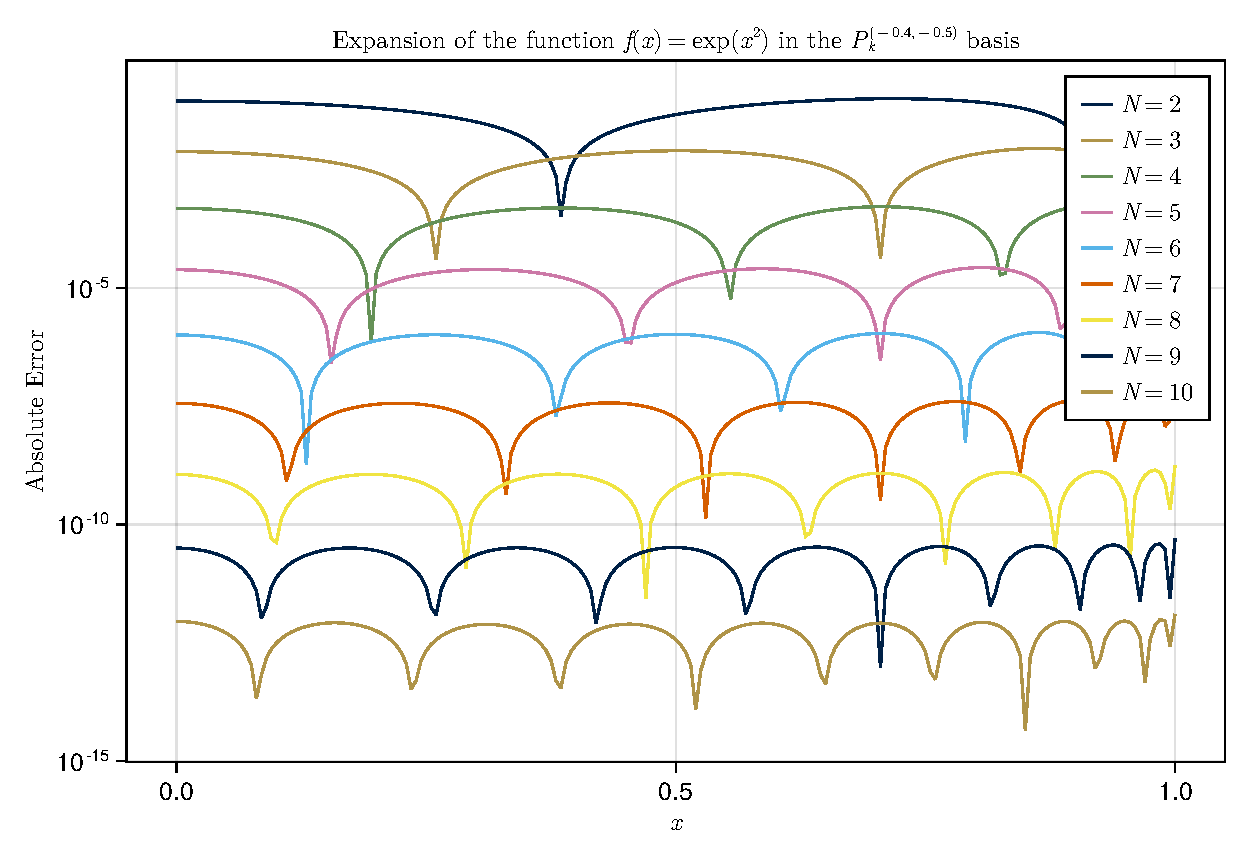
\includegraphics[width=0.7\linewidth]{results/jacobi-expansions.pdf}
  \caption[Convergence of Jacobi basis expansion]{Convergence of the Jacobi polynomial expansion $f_N(x) = \sum_{k=0}^{N-1} P_k^{(a, b)}(x)$ of an example function $f(x) = \e^{x^2}$ with $a = -\frac{3}{4}$ and $b = -\frac{1}{2}$. Each added term improves the absolute error between the function and its expansion by a factor, so we have exponential convergence. The number of ``arches'' of each solution error function, occuring from the roots of $f(x) - f_N(x)$, approximately equals the order $N$.}
\end{figure}

% TODO: Convergence speed according to theory is...?
